The main aim of Experiment 3 was to see whether vagueness would exert beneficial effects when all conditions used numerals in the instructions, and when there were vague and crisp versions of the instructions for both comparison and matching strategies. The main changes from Experiment 2 were that the human selection task was explicitly controlled (i.e., in whether it amounted to matching or comparison), and that all conditions were constrained to mention a number. We used the same arrays as in Experiment 2. Table \ref{Instructions for e3} shows the instructions for each condition. Note the difference between ``fewer than 20'' and ``far fewer than 20'': whereas the former cannot have borderline cases (i.e., for each number it is clear whether the number is smaller than 20 or not), the latter can.

\begin{table}
\centering
\caption{Experiment 3: Instructions arranged by condition for stimuli with $(6,15,24)$ dots and instructions indicating the smaller numbers} 
\label{Instructions for e3}
\begin{tabular}{cccc}
\hline\noalign{\smallskip}
Instruction	format          &Vagueness					&	Selection task	& Instruction									\\
\noalign{\smallskip}\hline\noalign{\smallskip}
\multirow{4}{*}{numeric}	&\multirow{2}{*}{crisp} 	&	matching		& Choose a square with 6 dots 					\\ 
							&							&	comparison 		& Choose a square with fewer than 20 dots 		\\
                             \cline{2-4}
							&\multirow{2}{*}{vague} 	&	matching 		& Choose a square with about 10 dots 			\\ 
							&							&	comparison 		& Choose a square with far fewer than 20 dots 	\\ 
\noalign{\smallskip}\hline
\end{tabular}
\end{table}%

\subsection{Hypotheses} % E 3
\noindent For Experiment 3, we hypothesised:

\begin{description}
	\item [Hypothesis 1] Vague instructions are easier for the reader than crisp ones (main effect of vagueness)
	\item [Hypothesis 2] Comparison is easier for the reader than matching (main effect of selection task)
	\item [Hypothesis 3] Effects of vagueness are different depending on whether the selection task is matching or comparison (interaction effect selection x vagueness).
\end{description}

\subsection{Experimental Method} % E 3

38 participants were recruited. We used a 2 x 2 factorial manipulation of vagueness and selection task (see Table \ref{Instructions for e3}).
On each trial an instruction was presented: participants pressed a key to dismiss the instruction, when the dot arrays were presented until the participant responded, and the response time and choice were recorded.

\subsection{Results} % E 3

We used the method proposed by \citet{Levy:MainEffectsInteractions} to test for the main effect of Vagueness in the presence of its higher-order interactions.

Response times were trimmed at 2.5 SD separately for each subject, leading to the loss of 204 trials (2.8\% of the trials).
Condition means for the remaining (logged) RTs are plotted in Figure \ref{resultse3}.
A linear mixed model was constructed for the logged response times, 
with sum-coded vagueness, instruction format, (and their interaction), and item as fixed effects, and the same effects as slopes over participant for random effects.

\begin{figure}[htbp]
\centering
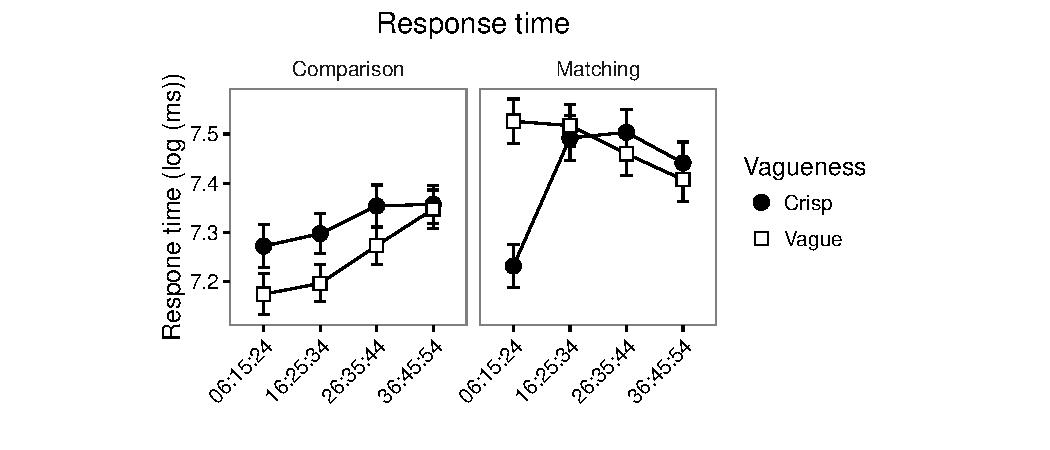
\includegraphics[width=\textwidth]{figures/e3-rtplot-1.pdf}
\caption{Mean response times by condition for Experiment 3 where all instructions were numeric}
\label{resultse3}
\end{figure}

\begin{description}
	\item [Test of Hypothesis 1] Vague instructions were non-significantly easier for the reader than crisp instructions when vagueness was considered as a main effect ($\beta=-0.01$, $se=0.01$, $t=-0.4$, $p=0.7158$). 
	\item [Test of Hypothesis 2] There was a statistically significant main effect of selection task, with the comparison task speeding responses compared to the matching task ($\beta=0.16$, $se=0.03$, $t=6.2$, $p<0.0001$). 
	\item [Test of Hypothesis 3] Vagueness exerted effects in different directions for the comparison task and for the matching task: there was a significant interaction between vagueness and selection task ($\beta=0.13$, $se=0.03$, $t=4.2$, $p<0.0001$). 
Separate analyses were conducted testing for effects of vagueness at each level of the selection task.
Within the comparison task vagueness significantly speeded response times compared with crisp controls ($\beta=-0.07$, $se=0.02$, $t=-3.5$, $p<0.0012$). 
Within the matching task vagueness significantly \emph{slowed} response times compared with crisp controls ($\beta=0.06$, $se=0.02$, $t=2.9$, $p<0.0061$). 
\end{description}

In other words, the cost reduction account was wrong to predict significant main effect advantages for vagueness (although there was a non-significant trend in the \emph{direction} predicted by the cost reduction account), and wrong to predict that vagueness should be beneficial at each level of the selection task: however vagueness was significantly advantageous in the comparison task.
